\documentclass[12pt]{article}

% Idioma y codificación
\usepackage[spanish, es-tabla]{babel}       %es-tabla para que se titule "Tabla"
\usepackage[utf8]{inputenc}

% Márgenes
\usepackage[a4paper,top=3cm,bottom=2.5cm,left=3cm,right=3cm]{geometry}

% Comentarios de bloque
\usepackage{verbatim}

% Paquetes de links
\usepackage[hidelinks]{hyperref}    % Permite enlaces
\usepackage{url}                    % redirecciona a la web

% Más opciones para enumeraciones
\usepackage{enumitem}

% Personalizar la portada
\usepackage{titling}


% Paquetes de tablas
\usepackage{multirow}


%------------------------------------------------------------------------

%Paquetes de figuras
\usepackage{caption}
\usepackage{subcaption} % Figuras al lado de otras
\usepackage{float}      % Poner figuras en el sitio indicado H.


% Paquetes de imágenes
\usepackage{graphicx}       % Paquete para añadir imágenes
\usepackage{transparent}    % Para manejar la opacidad de las figuras

% Paquete para usar colores
\usepackage[dvipsnames]{xcolor}
\usepackage{pagecolor}      % Para cambiar el color de la página

% Habilita tamaños de fuente mayores
\usepackage{fix-cm}


%------------------------------------------------------------------------

% Paquetes de matemáticas
\usepackage{mathtools, amsfonts, amssymb, mathrsfs}
\usepackage[makeroom]{cancel}     % Simplificar tachando
\usepackage{polynom}    % Divisiones y Ruffini
\usepackage{units} % Para poner fracciones diagonales con \nicefrac

\usepackage{pgfplots}   %Representar funciones
\pgfplotsset{compat=1.18}  % Versión 1.18

\usepackage{tikz-cd}    % Para usar diagramas de composiciones
\usetikzlibrary{calc}   % Para usar cálculo de coordenadas en tikz

%Definición de teoremas, etc.
\usepackage{amsthm}
%\swapnumbers   % Intercambia la posición del texto y de la numeración

\theoremstyle{plain}

\makeatletter
\@ifclassloaded{article}{
  \newtheorem{teo}{Teorema}[section]
}{
  \newtheorem{teo}{Teorema}[chapter]  % Se resetea en cada chapter
}
\makeatother

\newtheorem{coro}{Corolario}[teo]           % Se resetea en cada teorema
\newtheorem{prop}[teo]{Proposición}         % Usa el mismo contador que teorema
\newtheorem{lema}[teo]{Lema}                % Usa el mismo contador que teorema

\theoremstyle{remark}
\newtheorem*{observacion}{Observación}

\theoremstyle{definition}

\makeatletter
\@ifclassloaded{article}{
  \newtheorem{definicion}{Definición} [section]     % Se resetea en cada chapter
}{
  \newtheorem{definicion}{Definición} [chapter]     % Se resetea en cada chapter
}
\makeatother

\newtheorem*{notacion}{Notación}
\newtheorem*{ejemplo}{Ejemplo}
\newtheorem*{ejercicio*}{Ejercicio}             % No numerado
\newtheorem{ejercicio}{Ejercicio} [section]     % Se resetea en cada section


% Modificar el formato de la numeración del teorema "ejercicio"
\renewcommand{\theejercicio}{%
  \ifnum\value{section}=0 % Si no se ha iniciado ninguna sección
    \arabic{ejercicio}% Solo mostrar el número de ejercicio
  \else
    \thesection.\arabic{ejercicio}% Mostrar número de sección y número de ejercicio
  \fi
}


% \renewcommand\qedsymbol{$\blacksquare$}         % Cambiar símbolo QED
%------------------------------------------------------------------------

% Paquetes para encabezados
\usepackage{fancyhdr}
\pagestyle{fancy}
\fancyhf{}

\newcommand{\helv}{ % Modificación tamaño de letra
\fontfamily{}\fontsize{12}{12}\selectfont}
\setlength{\headheight}{15pt} % Amplía el tamaño del índice


%\usepackage{lastpage}   % Referenciar última pag   \pageref{LastPage}
\fancyfoot[C]{\thepage}

%------------------------------------------------------------------------

% Conseguir que no ponga "Capítulo 1". Sino solo "1."
\makeatletter
\@ifclassloaded{book}{
  \renewcommand{\chaptermark}[1]{\markboth{\thechapter.\ #1}{}} % En el encabezado
    
  \renewcommand{\@makechapterhead}[1]{%
  \vspace*{50\p@}%
  {\parindent \z@ \raggedright \normalfont
    \ifnum \c@secnumdepth >\m@ne
      \huge\bfseries \thechapter.\hspace{1em}\ignorespaces
    \fi
    \interlinepenalty\@M
    \Huge \bfseries #1\par\nobreak
    \vskip 40\p@
  }}
}
\makeatother

%------------------------------------------------------------------------
% Paquetes de cógido
\usepackage{minted}
\renewcommand\listingscaption{Código fuente}

\usepackage{fancyvrb}
% Personaliza el tamaño de los números de línea
\renewcommand{\theFancyVerbLine}{\small\arabic{FancyVerbLine}}

% Estilo para C++
\newminted{cpp}{
    frame=lines,
    framesep=2mm,
    baselinestretch=1.2,
    linenos,
    escapeinside=||
}



\usepackage{listings} % Para incluir código desde un archivo

\renewcommand\lstlistingname{Código Fuente}
\renewcommand\lstlistlistingname{Índice de Códigos Fuente}

% Definir colores
\definecolor{vscodepurple}{rgb}{0.5,0,0.5}
\definecolor{vscodeblue}{rgb}{0,0,0.8}
\definecolor{vscodegreen}{rgb}{0,0.5,0}
\definecolor{vscodegray}{rgb}{0.5,0.5,0.5}
\definecolor{vscodebackground}{rgb}{0.97,0.97,0.97}
\definecolor{vscodelightgray}{rgb}{0.9,0.9,0.9}

% Configuración para el estilo de C similar a VSCode
\lstdefinestyle{vscode_C}{
  backgroundcolor=\color{vscodebackground},
  commentstyle=\color{vscodegreen},
  keywordstyle=\color{vscodeblue},
  numberstyle=\tiny\color{vscodegray},
  stringstyle=\color{vscodepurple},
  basicstyle=\scriptsize\ttfamily,
  breakatwhitespace=false,
  breaklines=true,
  captionpos=b,
  keepspaces=true,
  numbers=left,
  numbersep=5pt,
  showspaces=false,
  showstringspaces=false,
  showtabs=false,
  tabsize=2,
  frame=tb,
  framerule=0pt,
  aboveskip=10pt,
  belowskip=10pt,
  xleftmargin=10pt,
  xrightmargin=10pt,
  framexleftmargin=10pt,
  framexrightmargin=10pt,
  framesep=0pt,
  rulecolor=\color{vscodelightgray},
  backgroundcolor=\color{vscodebackground},
}

%------------------------------------------------------------------------

% Comandos definidos
\newcommand{\bb}[1]{\mathbb{#1}}
\newcommand{\cc}[1]{\mathcal{#1}}

% I prefer the slanted \leq
\let\oldleq\leq % save them in case they're every wanted
\let\oldgeq\geq
\renewcommand{\leq}{\leqslant}
\renewcommand{\geq}{\geqslant}

% Si y solo si
\newcommand{\sii}{\iff}

% Letras griegas
\newcommand{\eps}{\epsilon}
\newcommand{\veps}{\varepsilon}
\newcommand{\lm}{\lambda}

\newcommand{\ol}{\overline}
\newcommand{\ul}{\underline}
\newcommand{\wt}{\widetilde}
\newcommand{\wh}{\widehat}

\let\oldvec\vec
\renewcommand{\vec}{\overrightarrow}

% Derivadas parciales
\newcommand{\del}[2]{\frac{\partial #1}{\partial #2}}
\newcommand{\Del}[3]{\frac{\partial^{#1} #2}{\partial^{#1} #3}}
\newcommand{\deld}[2]{\dfrac{\partial #1}{\partial #2}}
\newcommand{\Deld}[3]{\dfrac{\partial^{#1} #2}{\partial^{#1} #3}}


\newcommand{\AstIg}{\stackrel{(\ast)}{=}}
\newcommand{\Hop}{\stackrel{L'H\hat{o}pital}{=}}

\newcommand{\red}[1]{{\color{red}#1}} % Para integrales, destacar los cambios.

% Método de integración
\newcommand{\MetInt}[2]{
    \left[\begin{array}{c}
        #1 \\ #2
    \end{array}\right]
}

% Declarar aplicaciones
% 1. Nombre aplicación
% 2. Dominio
% 3. Codominio
% 4. Variable
% 5. Imagen de la variable
\newcommand{\Func}[5]{
    \begin{equation*}
        \begin{array}{rrll}
            #1:& #2 & \longrightarrow & #3\\
               & #4 & \longmapsto & #5
        \end{array}
    \end{equation*}
}

%------------------------------------------------------------------------

\lstset{
    basicstyle=\ttfamily,
    breaklines=true,
    breakatwhitespace=false,
    prebreak=\mbox{\textcolor{red}{$\hookleftarrow$}},
    postbreak=\mbox{\textcolor{red}{$\hookrightarrow$}},
    breakindent=1cm,
    literate={@}{@}{1\discretionary{}{}{}}
}

\begin{document}

    % 1. Foto de fondo
    % 2. Título
    % 3. Encabezado Izquierdo
    % 4. Color de fondo
    % 5. Coord x del titulo
    % 6. Coord y del titulo
    % 7. Fecha

    
    % 1. Foto de fondo
% 2. Título
% 3. Encabezado Izquierdo
% 4. Color de fondo
% 5. Coord x del titulo
% 6. Coord y del titulo
% 7. Fecha

\newcommand{\portada}[7]{

    \portadaBase{#1}{#2}{#3}{#4}{#5}{#6}{#7}
    \portadaBook{#1}{#2}{#3}{#4}{#5}{#6}{#7}
}

\newcommand{\portadaExamen}[7]{

    \portadaBase{#1}{#2}{#3}{#4}{#5}{#6}{#7}
    \portadaArticle{#1}{#2}{#3}{#4}{#5}{#6}{#7}
}




\newcommand{\portadaBase}[7]{

    % Tiene la portada principal y la licencia Creative Commons
    
    % 1. Foto de fondo
    % 2. Título
    % 3. Encabezado Izquierdo
    % 4. Color de fondo
    % 5. Coord x del titulo
    % 6. Coord y del titulo
    % 7. Fecha
    
    
    \thispagestyle{empty}               % Sin encabezado ni pie de página
    \newgeometry{margin=0cm}        % Márgenes nulos para la primera página
    
    
    % Encabezado
    \fancyhead[L]{\helv #3}
    \fancyhead[R]{\helv \nouppercase{\leftmark}}
    
    
    \pagecolor{#4}        % Color de fondo para la portada
    
    \begin{figure}[p]
        \centering
        \transparent{0.3}           % Opacidad del 30% para la imagen
        
        \includegraphics[width=\paperwidth, keepaspectratio]{assets/#1}
    
        \begin{tikzpicture}[remember picture, overlay]
            \node[anchor=north west, text=white, opacity=1, font=\fontsize{60}{90}\selectfont\bfseries\sffamily, align=left] at (#5, #6) {#2};
            
            \node[anchor=south east, text=white, opacity=1, font=\fontsize{12}{18}\selectfont\sffamily, align=right] at (9.7, 3) {\textbf{\href{https://losdeldgiim.github.io/}{Los Del DGIIM}}};
            
            \node[anchor=south east, text=white, opacity=1, font=\fontsize{12}{15}\selectfont\sffamily, align=right] at (9.7, 1.8) {Doble Grado en Ingeniería Informática y Matemáticas\\Universidad de Granada};
        \end{tikzpicture}
    \end{figure}
    
    
    \restoregeometry        % Restaurar márgenes normales para las páginas subsiguientes
    \pagecolor{white}       % Restaurar el color de página
    
    
    \newpage
    \thispagestyle{empty}               % Sin encabezado ni pie de página
    \begin{tikzpicture}[remember picture, overlay]
        \node[anchor=south west, inner sep=3cm] at (current page.south west) {
            \begin{minipage}{0.5\paperwidth}
                \href{https://creativecommons.org/licenses/by-nc-nd/4.0/}{
                    
\includegraphics[height=2cm]{assets/Licencia.png}
                }\vspace{1cm}\\
                Esta obra está bajo una
                \href{https://creativecommons.org/licenses/by-nc-nd/4.0/}{
                    Licencia Creative Commons Atribución-NoComercial-SinDerivadas 4.0 Internacional (CC BY-NC-ND 4.0).
                }\\
    
                Eres libre de compartir y redistribuir el contenido de esta obra en cualquier medio o formato, siempre y cuando des el crédito adecuado a los autores originales y no persigas fines comerciales. 
            \end{minipage}
        };
    \end{tikzpicture}
    
    
    
    % 1. Foto de fondo
    % 2. Título
    % 3. Encabezado Izquierdo
    % 4. Color de fondo
    % 5. Coord x del titulo
    % 6. Coord y del titulo
    % 7. Fecha


}


\newcommand{\portadaBook}[7]{

    % 1. Foto de fondo
    % 2. Título
    % 3. Encabezado Izquierdo
    % 4. Color de fondo
    % 5. Coord x del titulo
    % 6. Coord y del titulo
    % 7. Fecha

    % Personaliza el formato del título
    \pretitle{\begin{center}\bfseries\fontsize{42}{56}\selectfont}
    \posttitle{\par\end{center}\vspace{2em}}
    
    % Personaliza el formato del autor
    \preauthor{\begin{center}\Large}
    \postauthor{\par\end{center}\vfill}
    
    % Personaliza el formato de la fecha
    \predate{\begin{center}\huge}
    \postdate{\par\end{center}\vspace{2em}}
    
    \title{#2}
    \author{\href{https://losdeldgiim.github.io/}{Los Del DGIIM}}
    \date{Granada, #7}
    \maketitle
    
    \tableofcontents
}




\newcommand{\portadaArticle}[7]{

    % 1. Foto de fondo
    % 2. Título
    % 3. Encabezado Izquierdo
    % 4. Color de fondo
    % 5. Coord x del titulo
    % 6. Coord y del titulo
    % 7. Fecha

    % Personaliza el formato del título
    \pretitle{\begin{center}\bfseries\fontsize{42}{56}\selectfont}
    \posttitle{\par\end{center}\vspace{2em}}
    
    % Personaliza el formato del autor
    \preauthor{\begin{center}\Large}
    \postauthor{\par\end{center}\vspace{3em}}
    
    % Personaliza el formato de la fecha
    \predate{\begin{center}\huge}
    \postdate{\par\end{center}\vspace{5em}}
    
    \title{#2}
    \author{\href{https://losdeldgiim.github.io/}{Los Del DGIIM}}
    \date{Granada, #7}
    \thispagestyle{empty}               % Sin encabezado ni pie de página
    \maketitle
    \vfill
}
    \portadaExamen{etsiitA4.jpg}{Modelos de\\Computación\\Práctica Lex}{Práctica Lex. MC.}{MidnightBlue}{-8}{28}{2024}{Arturo Olivares Martos\\Joaquín Avilés de la Fuente}


    \begin{abstract}
        En la presente memoria se detallará la práctica llevada a cabo en la asignatura de Modelos de Computación del tercer curso del Doble Grado en Ingeniería Informática y Matemáticas de la Universidad de Granada.
        En ella, hemos implementado un menú con diversas funciones para analizar un texto introducido por el usuario, el cual detallaremos más adelante en las distintas secciones de la memoria.
    \end{abstract}

    \newpage
    \section{Introducción}

    En nuestro caso, para no limitarnos a un único caso de uso, lo cual probablemente implicaría usar menos expresiones regulares, hemos decidido implementar un menú con diversas opciones que permiten al usuario analizar un texto introducido por él mismo. Esto proporciona así más versatilidad, a la vez que nos facilita la implementación de un mayor número de expresiones regulares.

    La funcionalidad del programa se puede probar de forma directa mediante el menú creado, o se puede tambiar probar por separado con cada programa. Además, hemos creado un archivo \verb|makefile| que permite que la ejecución sea más sencilla.

    Todos estos aspectos los explicaremos de forma detallada en cada una de las secciones de este artículo.

    \begin{observacion}
    Todos las rutas relativas que se proporcionan suponen que nos encontramos en la carpeta raíz de esta práctica.
    \end{observacion}

    \section{Comprobación de Números de Teléfono}

    Este analizador se encuentra en el archivo \verb|Telefonos/regex_tfno.l|. Para compilarlo, se debe ejecutar el siguiente comando:
    \begin{minted}[linenos=false]{shell-session}
        $ flex++ -o regex_tfno.cpp regex_tfno.l
        $ g++ -Wall -o regex_tfno regex_tfno.cpp -lfl
    \end{minted}

    Para ejecutarlo, se debe ejecutar el siguiente comando:
    \begin{minted}[linenos=false]{shell-session}
        $ ./regex_tfno <fichero>
    \end{minted}
    donde \verb|<fichero>| es el archivo que se desea analizar en busca de números de teléfono.
    De forma alternativa, se recomienda usar el \verb|makefile| proporcionado usando la siguiente regla:
    \begin{minted}[linenos=false]{shell-session}
        $ make telefonos
    \end{minted}
    En este caso, el archivo de texto que se analizará es \verb|Telefonos/telefonos.txt|, por lo que deberán almacenarse en ese archivo las cadenas que se deseen procesar.\\

    Este programa analiza el archivo pasado en búsqueda de números de teléfono. Por un lado, informa de las cadenas que no han sido identificadas con números de teléfono de ningún país registrado y, por otro lado, de los números de teléfono válidos que se han encontrado, informa en qué país son válidos. Actualmente tan solo se ha implementado la detección de números de teléfono españoles, puesto que son los que conocemos de primera mano, pero la extensión a otros países es directa.
    Para detectar los números de teléfono, se han usado las siguientes expresiones regulares:
    \begin{itemize}
        \item \ul{\texttt{tfno\_espanol\_grupos3}}:
        \begin{lstlisting}
((00|"+")34(" ")?)?([0-9]{3}(" ")?){3}
        \end{lstlisting}
        
        En este caso, se da la posibilidad a que el número de teléfono esté agrupado en grupos de 3 cifras, separados por un espacio. En primer lugar, puede comenzar con el prefijo internacional (\verb|34| en el caso de España), que ha de ir precedido de \verb|00| o \verb|+|. A continuación, se encuentras los tres grupos de 3 cifras, en total 9 cifras. Se permite que haya un espacio entre los grupos de cifras y tras el prefijo internacional.

        \item \ul{\texttt{tfno\_espanol\_grupos2}}:
        \begin{lstlisting}
((00|"+")34(" ")?)?([0-9]{3}(" ")?){1}([0-9]{2}(" ")?){3}
        \end{lstlisting}
        
        Esta expresión es similar, solo que permite que los 6 últimos finales se agrupen en tres grupos de 2 cifras, en lugar de dos grupos de 3 cifras. De nuevo, se permite que haya un espacio entre los grupos de cifras y tras el prefijo internacional (si lo hay).
    \end{itemize}

    Hemos limitado a estos casos, puesto que son los más habituales en España. No obstante, se podrían añadir más expresiones regulares para detectar otros formatos de números de teléfono. Tenemos por tanto la siguiente regla, la cual fuerza a que se cumpla una de las dos expresiones regulares anteriores, y esto sea lo único que se encuentre en la línea:
    \begin{minted}[
        fontsize=\footnotesize,
        linenos=false,
        breaklines=false
    ]
        {c++}
        ^{tfno_espanol_grupos3}|{tfno_espanol_grupos2}$   {tfno_pais["España"].insert(yytext);}
    \end{minted}
    Como vemos, los teléfonos detectados los almacenamos en un conjunto asociado a la clave \verb|España|, de forma que sería muy fácilmente generalizable a un mayor número de países. Un ejemplo de funcionamiento de este programa se encuentra en la Figura~\ref{fig:telefonos}.
    \begin{figure}
        \centering
        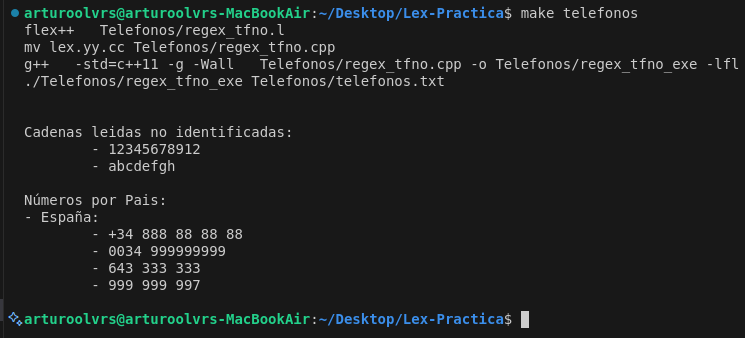
\includegraphics[width=\textwidth]{Img/Funcionamiento_Tfno.png}
        \caption{Ejemplo de ejecución del programa \texttt{regex\_tfno}.}
        \label{fig:telefonos}
    \end{figure}

    \section{Comprobación de Direcciones de Correo Electrónico}

    Este analizador se encuentra en el archivo \verb|EMAIL/regex_email.l|. Para compilarlo, se debe ejecutar el siguiente comando:
    \begin{minted}[linenos=false]{shell-session}
        $ flex++ -o regex_email.cpp regex_email.l
        $ g++ -Wall -o regex_email regex_email.cpp -lfl
    \end{minted}

    Para ejecutarlo, se debe ejecutar el siguiente comando:
    \begin{minted}[linenos=false]{shell-session}
        $ ./regex_email <fichero>
    \end{minted}
    donde \verb|<fichero>| es el archivo que se desea analizar en busca de direcciones de correo electrónico.

    De forma alternativa, se recomienda usar el \verb|makefile| proporcionado usando la siguiente regla:
    \begin{minted}[linenos=false]{shell-session}
        $ make email
    \end{minted}

    En este caso, el archivo de texto que se analizará es \verb|EMAIL/email.txt|, por lo que deberán almacenarse en ese archivo las cadenas que se deseen procesar.\\

    Este programa analiza el archivo pasado en búsqueda de direcciones de correo electrónico, informando cuáles son válidas y cuáles no. Respecto a la validación de correos, en internet hay gran cantidad de expresiones regulares disponibles, la mayoria de una alta complejidad que usan al RFC 3696, que es la documentación en la cual se especifica qué formato han de tener las direcciones de correo electrónico. No obstante hemos optado por una expresión regular más sencilla hecha por nosotros, la cual detecta la gran mayoria de correos electrónicos válidos en la actualidad. La expresión regular que hemos usado es la siguiente:
    \begin{lstlisting}
[a-zA-Z0-9]+((\.|-)?[a-zA-Z0-9]+)*@[0-9]*[a-zA-Z]+[a-zA-Z0-9]*\.(com|es|org)
    \end{lstlisting}

    Las limitaciones que esta expresión regular establece son:
    \begin{itemize}
        \item Distinguiremos entre la parte local (antes del @) y dominio (tras el @).
        \item Respecto a la parte local, ha de ser una sucesión de caracteres alfanuméricos junto a guiones y a puntos, teniendo en cuenta que:
        \begin{itemize}
            \item Ha de empezar y terminar por un caracter alfanumérico.
            \item Tras cada guion o punto ha de ir un carácter alfanumérico, de forma que no haya dos símbolos especiales consecutivos.
        \end{itemize}
        \item Respecto al dominio, antes del punto ha de haber una sucesión de caracteres alfanuméricos conteniendo al menos una letra, y tras el punto tan solo se admiten tres posibilidades: \verb|com|, \verb|es| u \verb|org|.
    \end{itemize}

    Somos conscientes de que esta expresión regular no es correcta (el correo electrónico institucional de la UGR no sería válido, por ejemplo), pero nos hemos limitado a ella para usar así una expresión regular legible. Un ejemplo de funcionamiento de este programa se encuentra en la Figura~\ref{fig:email}. Notemos que el correo \verb|correo@malo.com.| no se ha dado como válido puesto que está seguido justo de un punto, por lo que lo detecta como parte del dominio.
    \begin{figure}
        \centering
        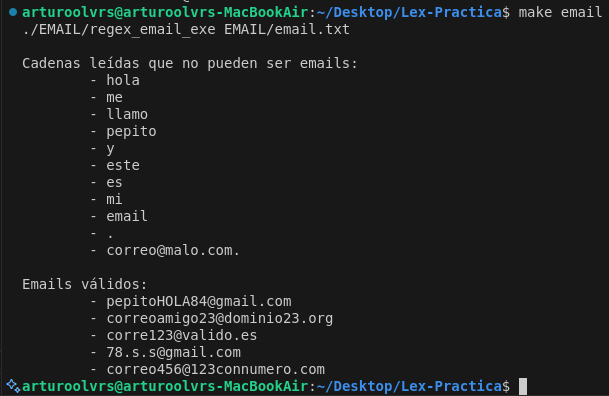
\includegraphics[width=\textwidth]{Img/Funcionamiento_Email.png}
        \caption{Ejemplo de ejecución del programa \texttt{regex\_email}.}
        \label{fig:email}
    \end{figure}

    \section{Comprobación de DNIs y de NIEs}

    Este analizador se encuentra en el archivo \verb|DNI-NIE/regex-dni-nie.l|. Para compilarlo, se debe ejecutar el siguiente comando:
    \begin{minted}[linenos=false]{shell-session}
        $ flex++ -o regex-dni-nie.cpp regex-dni-nie.l
        $ g++ -Wall -o regex-dni-nie regex-dni-nie.cpp -lfl
    \end{minted}

    Para ejecutarlo, se debe ejecutar el siguiente comando:
    \begin{minted}[linenos=false]{shell-session}
        $ ./regex-dni-nie <fichero>
    \end{minted}
    donde \verb|<fichero>| es el archivo que se desea analizar en busca de DNIs y NIEs.

    De forma alternativa, se recomienda usar el \verb|makefile| proporcionado usando la siguiente regla:
    \begin{minted}[linenos=false]{shell-session}
        $ make dni-nie
    \end{minted}

    En este caso, el archivo de texto que se analizará es \verb|DNI-NIE/dni-nie.txt|, por lo que deberán almacenarse en ese archivo las cadenas que se deseen procesar.\\

    Este programa analiza el archivo pasado en búsqueda de DNIs y NIEs, informando cuáles son válidos y cuáles no. La validación de DNIs y NIEs es más compleja, ya que por un lado se buscan aquellos candidatos a ser válidos (los que cumplan una expresión regular concreta, que explicaremos a continuación) y, por otro lado, ha de comprobarse que la letra del DNI o NIE sea la correcta. Respecto al patrón que han de seguir para poder ser válidos, hemos usado las siguientes expresiones regulares:
    \begin{itemize}
        \item \ul{Para los DNIs}:
        \begin{lstlisting}
[0-9]{8}(" "|"-")?[A-Z]
        \end{lstlisting}
        
        Como el lector sabe, el DNI está formado por 8 dígitos seguidos de una letra en mayúsuculas. Se permite que haya un espacio o un guión tras los 8 dígitos.

        \item \ul{Para los NIEs}:
        \begin{lstlisting}
[XYZ](" "|"-")?[0-9]{7}(" "|"-")?[A-Z]
        \end{lstlisting}
        
        En este caso, el NIE puede empezar por una X, Y o Z, seguido de 7 dígitos y una letra en mayúsculas. De nuevo, se permite que haya un espacio o un guión antes y tras los dígitos.
    \end{itemize}

    Las reglas que hemos usado para detectar DNIs y NIEs son sencillas, y se muestran a continuación:
    \begin{minted}[
        fontsize=\footnotesize,
        linenos=false,
        breaklines=false
    ]
        {c++}
        {DNI}       {dnis.push_back(yytext);}
        {NIE}       {nies.push_back(yytext);}
    \end{minted}

    De esta forma, se almacenan en dos vectores los DNIs y NIEs detectados, respectivamente. No obstante, llegados a este punto tenemos los que pueden ser válidos, pero no se ha probado su validez, puesto que falta comprobar el dígito de control. Esta comprobación se ha realizado siguiento la documentación oficial proporcionada por el \href{https://www.interior.gob.es/opencms/es/servicios-al-ciudadano/tramites-y-gestiones/dni/calculo-del-digito-de-control-del-nif-nie/}{Ministerio del Interior}.
    \begin{itemize}
        \item Para la comprobación de DNIs, la letra se calcula como el resto de dividir el número del DNI entre 23, y según ese resto se elije una letra concreta proporcionada por la web previamente mencionada. El DNI será válido si la letra que se ha calculado es la misma que la que se ha introducido.
        \item Para la comprobación de NIEs, se sustituye la X, Y o Z iniciales por un $0$, $1$ o $2$, respectivamente, y se sigue el mismo procedimiento que para los DNIs.
    \end{itemize}

    De esta forma, se puede comprobar si un DNI o NIE es válido o no. Un ejemplo de funcionamiento de este programa se encuentra en la Figura~\ref{fig:dni-nie}. Como vemos, aunque haya una gran cantidad de DNIs reconocidos como tal, la mayoría de ellos no son válidos tras comprobarlos con el dígito de control.
    \begin{figure}
        \centering
        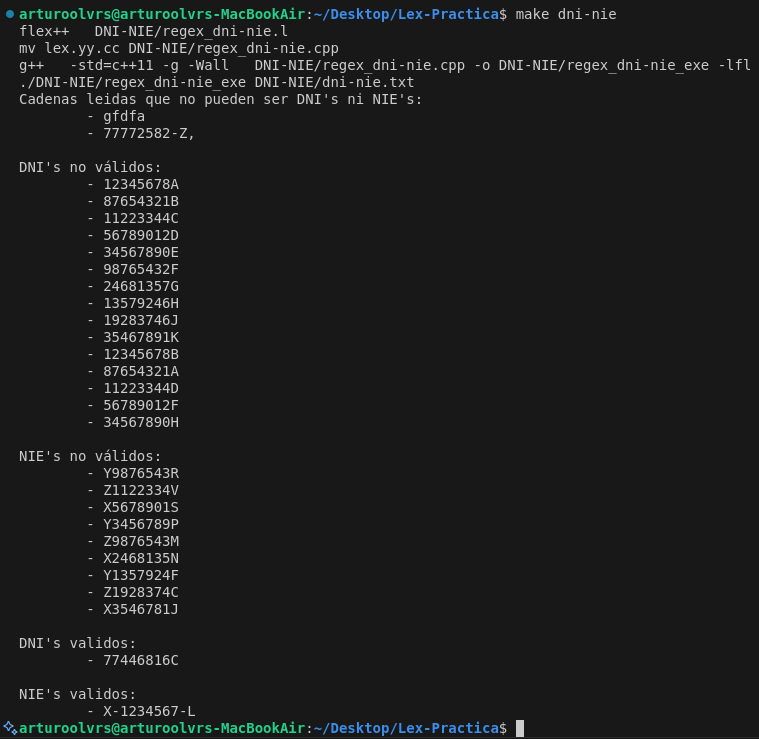
\includegraphics[width=\textwidth]{Img/Funcionamiento_DNI-NIE.png}
        \caption{Ejemplo de ejecución del programa \texttt{regex-dni-nie}.}
        \label{fig:dni-nie}
    \end{figure}

    \section{Comprobación de Cuentas Bancarias}

    Este analizador se encuentra en el archivo \verb|Bancos/regex_bancos.l|. Para compilarlo, se debe ejecutar el siguiente comando:
    \begin{minted}[linenos=false]{shell-session}
        $ flex++ -o regex_bancos.cpp regex_bancos.l
        $ g++ -Wall -o regex_bancos regex_bancos.cpp -lfl
    \end{minted}

    Para ejecutarlo, se debe ejecutar el siguiente comando:
    \begin{minted}[linenos=false]{shell-session}
        $ ./regex_bancos <fichero>
    \end{minted}
    donde \verb|<fichero>| es el archivo que se desea analizar en busca de cuentas bancarias.

    De forma alternativa, se recomienda usar el \verb|makefile| proporcionado usando la siguiente regla:
    \begin{minted}[linenos=false]{shell-session}
        $ make bancos
    \end{minted}

    En este caso, el archivo de texto que se analizará es \verb|Bancos/bancos.txt|, por lo que deberán almacenarse en ese archivo las cadenas que se deseen procesar.\\

    Este programa analiza el archivo pasado en búsqueda de cuentas bancarias, informando finalmente la entidad bancaria a la que corresponde cada cuenta. En primer lugar, hemos de tener en cuenta que se restringe a las cuentas bancarias españolas, ya que es el único país cuyas cuentas bancarias conocemos. Tras detectar las cuentas bancarias mediante una expresión regular que más adelante se detallará, estas se validan también mediante dos dígitos de control de forma similar a los DNIs, y finalmente, de las cuentas bancarias válidas, informamos de su entidad bancaria.

    La expresión regular que hemos usado para detectar cuentas bancarias españolas es la siguiente:
    \begin{lstlisting}
ES[0-9]{2}(" "[0-9]{4}){5}
    \end{lstlisting}

    En este caso, el IBAN de la cuenta bancaria ha de empezar por \verb|ES| (por ser españolas), seguido de dos dígitos (serán los dígitos de control), y a continuación 5 grupos de 4 dígitos separados por un espacio, que componen el número de cuenta. De todas estas cuentas (que son las candidatas a ser válidas), se ha de comprobar que los dígitos de control sean correctos. Para ello, se ha usado la documentación oficial proporcionada por el \href{https://clientebancario.bde.es/pcb/es/blog/que-se-esconde-tras-los-numeros-de-tu-cuenta-corriente-.html}{Banco de España}, que proporciona una serie de pasos a seguir para comprobar la validez de una cuenta bancaria. En resumen, se han de seguir los siguientes pasos:
    \begin{enumerate}
        \item Se toman los $20$ dígitos que forman el número de cuenta (excluyendo las letras del país, ``ES'', y los dos dígitos de control).
        \item Tras ellos, para cada letra del código del país, se le asigna un número. A la A se le asigna el $10$, a la B el $11$, y así sucesivamente hasta la Z. En el caso de ``ES'', se le asigna el $14$ y el $28$, y ambos se añaden al final de los $20$ dígitos.
        \item Por último, y como desconocemos los dos dígitos de control (queremos calcularlos), se añaden al final dos ceros.
        \item A este número obtenido (con $26$ cifras\footnote{Este aspecto hay que tenerlo en cuenta a la hora de calcular el resto, puesto que no se puede almacenar entero en un tipo de dato numérico de \texttt{C++}.}) se le calcula el resto de dividirlo entre $97$.
        \item A $98$ se le resta el resto obtenido, y este resultado (que será de dos cifras (pudiendo ser el primero un $0$)) será el número de control. Estos dos dígitos han de ser los mismos que los dos dígitos de control que se han introducido para que el IBAN sea válido.
    \end{enumerate}

    Una vez validados los IBAN, buscamos informar de la entidad bancaria a la que pertenecen. Para ello, hemos usado también la información oficial del Banco de España, ya que los primeros 4 dígitos tras los dígitos de control corresponden a la entidad bancaria. En la documentación proporcionada por el Banco de España, se detalla qué entidad bancaria corresponde a cada número, y hemos usado esta información para informar al usuario de la entidad bancaria a la que pertenece la cuenta bancaria. Un ejemplo de funcionamiento de este programa se encuentra en la Figura~\ref{fig:bancos}.
    \begin{figure}
        \centering
        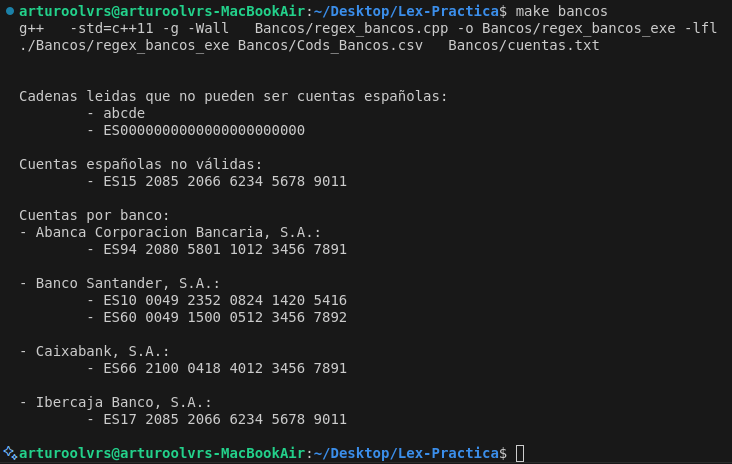
\includegraphics[width=\textwidth]{Img/Funcionamiento_Bancos.png}
        \caption{Ejemplo de ejecución del programa \texttt{regex\_bancos}.}
        \label{fig:bancos}
    \end{figure}

    \section{Menú de Opciones}

    Llegados a este punto, en el que hemos explicado cada una de las distintas funcionalidades que hemos implementado, vamos a explicar otra forma de probarlas, que es mediante el menú que hemos creado. Este menú se encuentra en el archivo \verb|menu.cpp|, y al no contener ningún comando de flex, se compila de la forma habitual:
    \begin{minted}[linenos=false]{shell-session}
        $ g++ -Wall -o menu menu.cpp
    \end{minted}

    Para ejecutarlo, se debe ejecutar el siguiente comando:
    \begin{minted}[linenos=false]{shell-session}
        $ ./menu
    \end{minted}

    De forma alternativa, se recomienda usar el \verb|makefile| proporcionado usando la siguiente regla:
    \begin{minted}[linenos=false]{shell-session}
        $ make menu
    \end{minted}

    Al ejecutar este programa, se mostrará un menú con las distintas opciones que se pueden elegir, y se podrá seleccionar la que se desee. Las opciones que se pueden elegir son las siguientes:
    \begin{enumerate}
        \item Comprobación de números de teléfono.
        \item Comprobación de direcciones de correo electrónico.
        \item Comprobación de DNIs y NIEs.
        \item Comprobación de cuentas bancarias.
    \end{enumerate}

    Una vez elegida cualquiera de las opciones, se pide por la entrada estándar al usuario que introduzca el texto que desea analizar, y este se le pasará al programa correspondiente. Un ejemplo de funcionamiento de este menú se encuentra en la Figura~\ref{fig:menu}.
    \begin{figure}
        \centering
        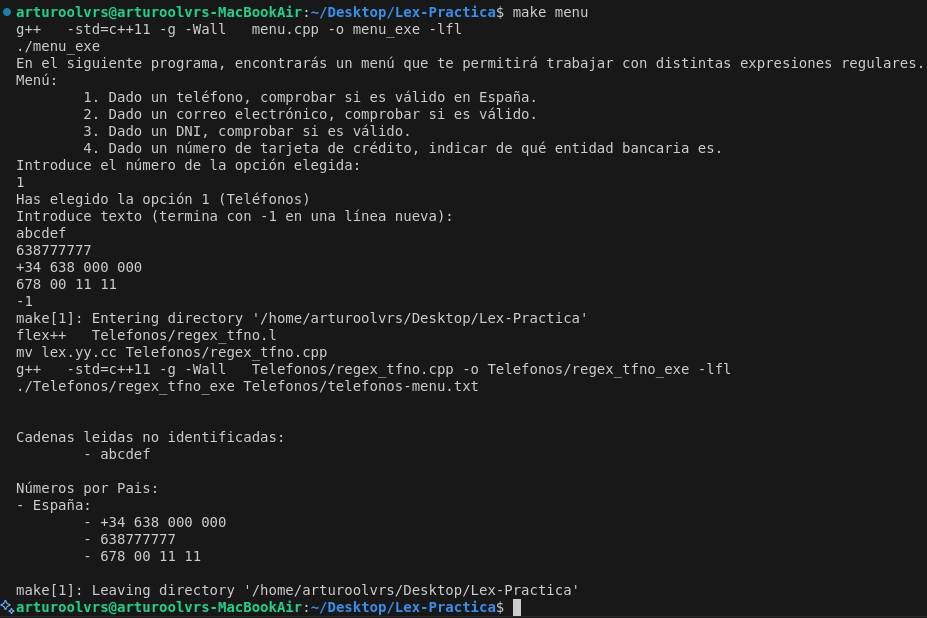
\includegraphics[width=\textwidth]{Img/Funcionamiento_Menu.png}
        \caption{Ejemplo de ejecución del menú.}
        \label{fig:menu}
    \end{figure}
\end{document}
